%%%%%%%%%%%%%%%%%%%%%%%%%%%%%%%%%%%%%%%%%
% Memo
% LaTeX Template
% Version 1.0 (30/12/13)
%
% This template has been downloaded from:
% http://www.LaTeXTemplates.com
%
% Original author:
% Rob Oakes (http://www.oak-tree.us) with modifications by:
% Vel (vel@latextemplates.com)
%
% License:
% CC BY-NC-SA 3.0 (http://creativecommons.org/licenses/by-nc-sa/3.0/)
%
%%%%%%%%%%%%%%%%%%%%%%%%%%%%%%%%%%%%%%%%%

\documentclass[a4paper,11pt]{../LatexDocStructures/MTItexMemo} % Set the paper size (letterpaper, a4paper, etc) and font size (10pt, 11pt or 12pt)

\usepackage{parskip} % Adds spacing between paragraphs
\setlength{\parindent}{15pt} % Indent paragraphs

\usepackage{xcolor}

\usepackage[dutch]{babel}
\usepackage{wrapfig}
\usepackage{hyperref} % Required for hyperlinks
\hypersetup{hidelinks,colorlinks,breaklinks=true,urlcolor=blue,citecolor=blue,linkcolor=blue,bookmarksopen=false}

\usepackage{titlesec}

\titlespacing\section{0pt}{12pt plus 4pt minus 2pt}{0pt plus 2pt minus 2pt}
\titlespacing\subsection{0pt}{6pt plus 2pt minus 2pt}{0pt plus 2pt minus 2pt}

%----------------------------------------------------------------------------------------
%	MEMO INFORMATION
%----------------------------------------------------------------------------------------

\memoto{Jeroen van Elburg; Richard Kaandorp} % Recipient(s)

\memocc{Mario Alvarez Grima; Wouter Bron; Jort van Wijk; Sergio Ooijens}

\memofrom{\href{https://nl.linkedin.com/in/jellespijker}{Jelle Spijker} ( \href{mailto:spijker.jelle@gmail.com}{spijker.jelle@gmail.com})} % Sender(s)

\memosubject{Machinaal scheiden van nat zand voor vision based verwerking } % Memo subject

\memodate{\today} % Date, set to \today for automatically printing todays date

\logo{
\includegraphics[width=0.2\textwidth]{../Pictures/MTI_logo.png}} % Institution logo at the top right of the memo, comment out this line for no logo

%----------------------------------------------------------------------------------------

\begin{document}

\maketitle % Print the memo header information
%----------------------------------------------------------------------------------------
%	MEMO CONTENT
%----------------------------------------------------------------------------------------
\section{Achtergrond}
\begin{wrapfigure}{r}{7.7cm}
	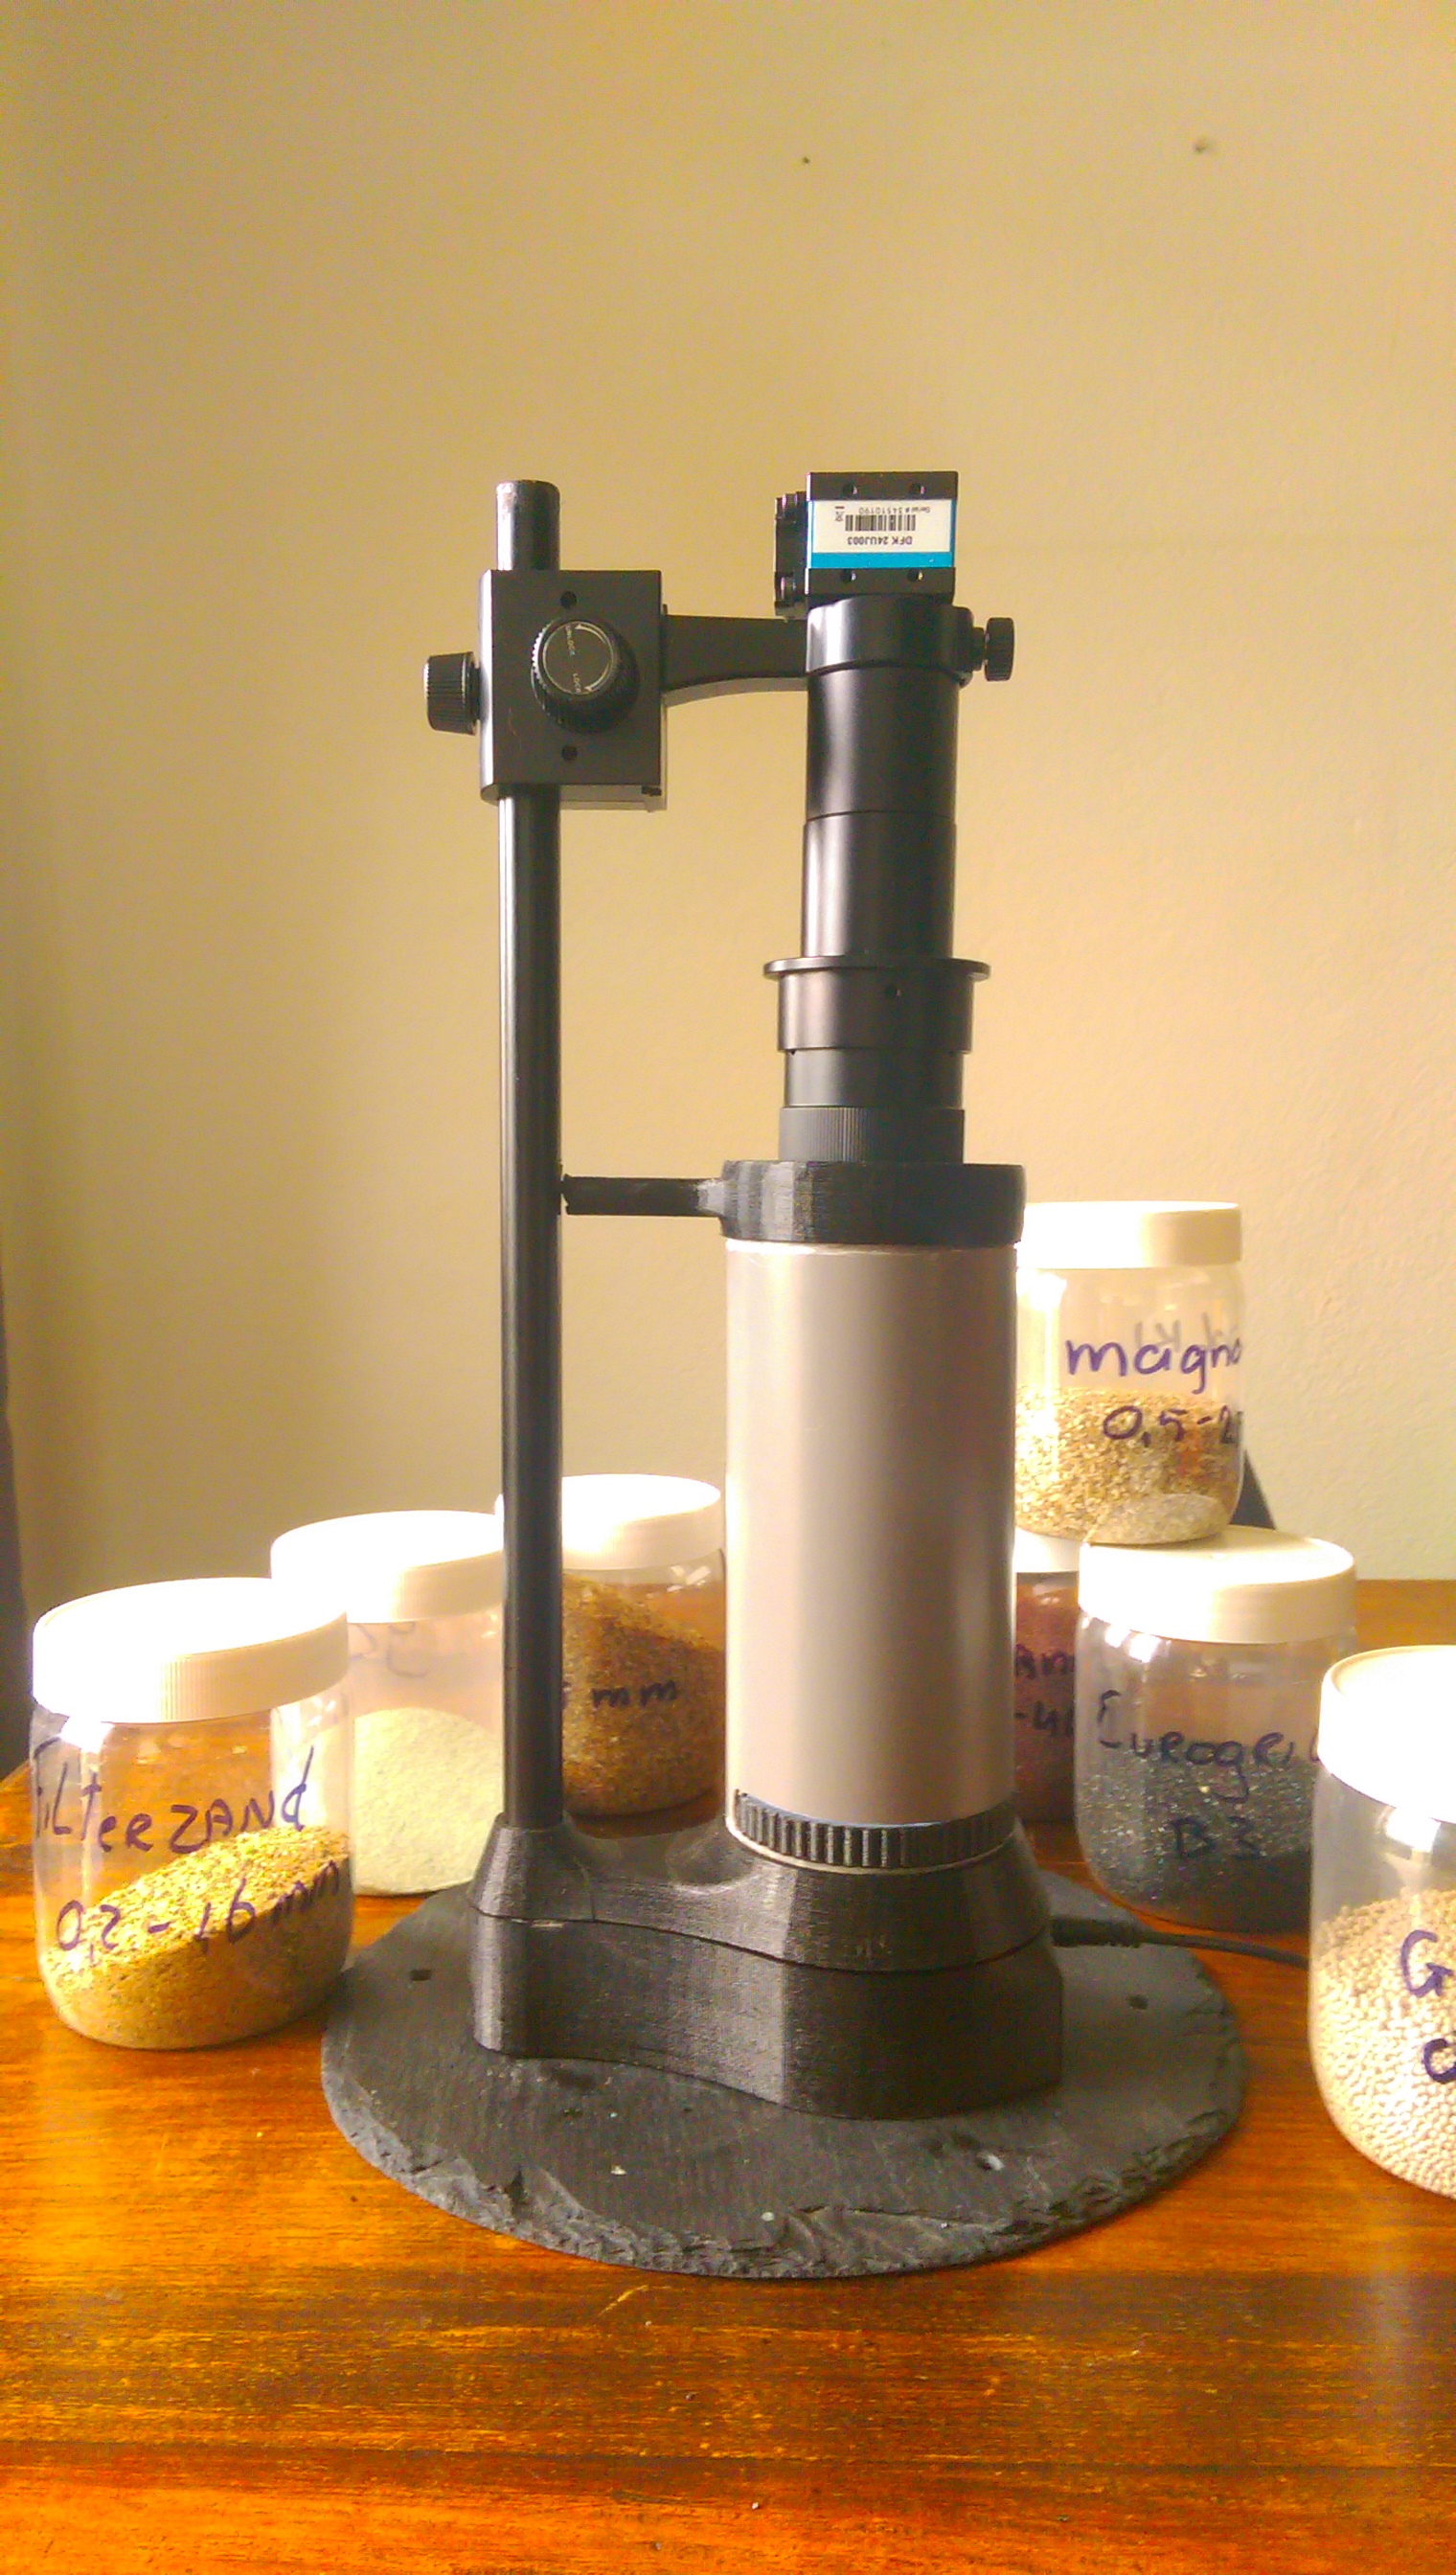
\includegraphics[width=7.7cm]{../Pictures/minorprototype.jpg}
	\caption{EVD prototype}
\end{wrapfigure}

Tijdens de minor embedded vision design (EVD) is een grond analyseer apparaat ontwikkeld. Deze analyseert gedroogde grondmonsters met behulp van een digitale camera en doet een uitspraak over kleur, structuur en textuur. Deze vision based sand analyzer (VSA) onderscheid zichzelf doordat hij handzaam en draagbaar is. hierdoor kan op locatie een grondmonster geanalyseerd worden. De meeste apparaten welke grond analyseren zijn log, groot, zwaar en staan daardoor in laboratoria.

Computer vision werkt met behulp van diverse algoritmes, deze identificeren interessante objecten in digitale beelden. Doordat de intensiteit van een pixel welke tot een object behoort afwijkt van achtergrond pixels kan een computer relevante objecten herkennen en segmenteren ten opzichte van de achtergrond. Hier worden additionele wiskundige operaties op uitgevoerd, zoals het bepalen van het oppervlak, omschrijven van kleur en classificeren van vorm. Resultaten van deze analyses zijn sterk afhankelijk van de kwaliteit van segmentatie proces.

De VSA wordt verder ontwikkeld tijdens een werktuigbouwkundige afstudeeropdracht in opdracht van IHC MTI B.V.. Een van de geïdentificeerde deelproblemen van deze opdracht is het analyseren van nat zand. Het is de bedoeling dat het apparaat direct in het veld gebruikt kan worden. Dit houdt in dat er met nat zand gewerkt kan en zal worden. Deze heeft als eigenschap dat korrels samen klonteren. Het water heeft namelijk een adhesive werking tussen korrels door van der Waals krachten. Deze samen geklonterde korrels worden door een digitale camera als een enkele korrel geregistreerd. Dit geeft een verstoring van statistische analyse. 

\section{Opdracht}
\noindent Ontwikkel een oplossing waarmee natte samengeklonterde grondkorrels door middel van mechanische actie gelijkmatig en in hoge mate gescheiden gepositioneerd worden in het zichtveld van een camera.
\begin{figure}[h]
	\centering
	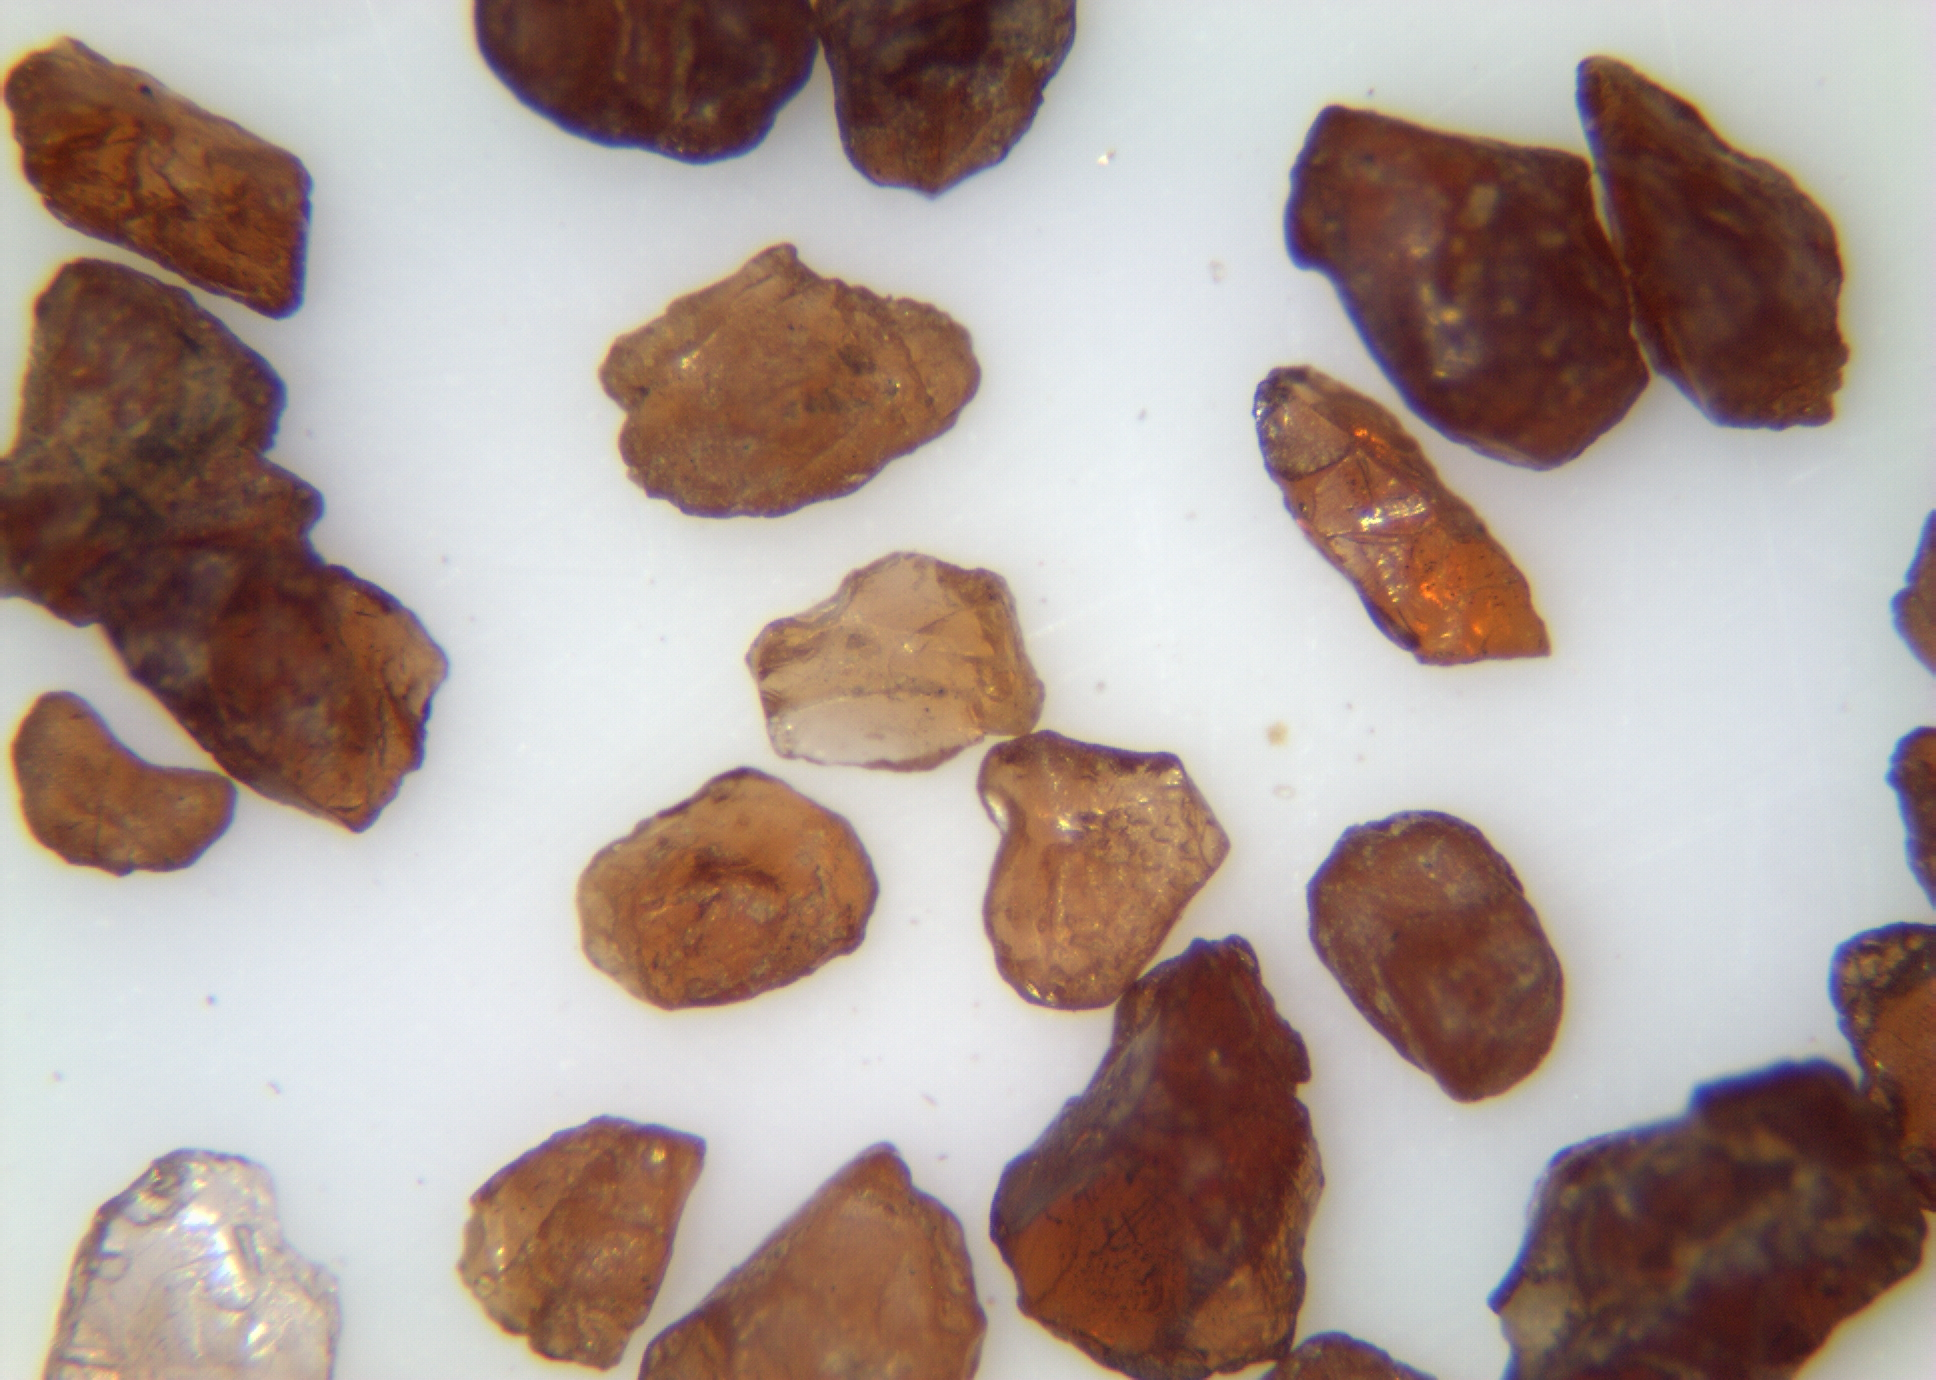
\includegraphics[width=10cm]{../Pictures/gannet2040.png}
	\caption{Droge zandkorrels $ 0.5 - 1 [mm] $ in doorsnede}
\end{figure}

\subsection{Zand specificatie}
\begin{description}
	\setlength{\itemsep}{0cm}
	\setlength{\parskip}{0cm}
	\item[\textbf{Aantal}] $ \pm 500 [korrel] $ natte grondkorrels.
	\item[\textbf{Dimensies}] Doorsnede $ 63[\mu m] $ tot $ 2 [mm] $.
	\item[\textbf{Materiaal}] Organische en anorganische deeltjes.
\end{description}
\subsection{Vision specificaties}
\begin{description}
	\setlength{\itemsep}{0cm}
	\setlength{\parskip}{0cm}
	\item[\textbf{Aantal}] Maximaal $ 15 [foto] $
	\item[\textbf{Belichtingstijd}] $ ^1/_6 [s] $
	\item[\textbf{Totale procestijd}] $ 60 [s] $
	\item[\textbf{Werkgebied}] Cirkel met $ D = 15 [mm] $
\end{description}

\subsection{Randvoorwaarden}
\begin{description}
	\setlength{\itemsep}{0cm}
	\setlength{\parskip}{0cm}
	\item Sign a Non Disclosure Agreement (\textbf{NDA})
\end{description}

\section{Bedrijfsprofiel}
IHC MTI B.V. heeft als basis Delftech park in Delft. Zij zijn wereldwijd het kenniscentrum voor het ontwikkelen van bagger, mijnbouw en diepzee mijnbouw specificaties, ontwerpen en ontwikkelingen van apparaten. MTI is een dochter onderneming van de Koninklijke IHC een wereldleider in de bouw van bagger- en marine \& offshore schepen.

MTI heeft ongeveer 60 man in dienst waaronder ervaren ingenieurs in de disciplines, dredging engineering, mining engineering, process engineering, mechanical engineering, fluid dynamic engineering, geophysics, geology, ship dynamics and design and multi-phase dynamics. 15\% bezit een doctorsgraad.\\
-----------------------------------------------------------------------------------------------------------------------------------

\noindent \textbf{Aanvullende informatie:} \href{https://sway.com/iI7d7AZ0BlfC2fIf}{Sway presentation}
%----------------------------------------------------------------------------------------

\end{document}